\documentclass[25pt, a0paper, landscape]{tikzposter}

% --- Packages ---
\usepackage[utf8]{inputenc}
\usepackage{amsmath, amssymb, amsthm}
\usepackage{mathtools}
\usepackage{enumitem}

\usepackage{etoolbox}
\usepackage{booktabs}
\usepackage{caption, tikz-cd}
\makeatletter
% Fixes the "There is no 1 in font nullfont" bug in tikzposter
\define@key{title}{titletextscale}{\def\TP@titletextscale{#1}}
\makeatother


% --- Poster Theme ---
\usetheme{Basic} % Options: Simple, Basic, Rays, Wave, etc.
\usecolorstyle{Default} % Can be customized for university colors

% --- Custom Math Commands (for p-adic groups) ---
\newcommand{\Fq}{\mathbb{F}_q}
\newcommand{\Fp}{\mathbb{F}_p}
\newcommand{\G}{\mathsf{G}}
\newcommand{\cB}{\mathcal{B}}
\newcommand{\SL}{\mathrm{SL}}
\newcommand{\Spin}{\mathrm{Spin}}
\newcommand{\Sp}{\mathrm{Sp}}
\newcommand{\SO}{\mathrm{SO}}
\newcommand{\PGSp}{\mathrm{PGSp}}
\newcommand{\FT}{\mathrm{FT}}
\newcommand{\un}{\mathrm{un}}
\newcommand{\res}{\mathrm{res}}
\newcommand{\cpt}{\mathrm{cpt}}



\newcommand{\CC}{\mathbb{C}}
\newcommand{\QQ}{\mathbb{Q}}
\newcommand{\ZZ}{\mathbb{Z}}

% Switch to the 'definition' style (Bold title, Upright text)
\theoremstyle{definition}
\newtheorem{theorem}{Theorem}
\newtheorem*{example}{Example}

% 3. Optional: Define other environments you might need
\newtheorem{definition}[theorem]{Definition}
\newtheorem{corollary}[theorem]{Corollary}
\newtheorem*{conjecture}{Conjecture}

% --- Title Data ---
\title{A nonabelian Fourier transform for unipotent representations of $p$-adic groups}
\author{Albert Lopez Bruch}
\institute{London School of Geometry and Number Theory}

\begin{document}

\maketitle

\begin{columns}
    % --- COLUMN 1: Introduction & Reduction ---
    \column{0.26}
    \block{Main Aims}{
        Find stable combinations of characters of unipotent representations of simple $p$-adic groups inside an $L$-packet.
    }
    \block{The $p$-adic groups}{
        \textbf{Reductive groups over a p-adic field} (commonly denoted as $p$-adic groups) are certain subgroups of $GL_n(F)$ with ``nice" structural and representation-theoretic properties, where $F$ is a finite extension of $\mathbb{Q}_p$. We assume that the $p$-adic group $G$ is simple and split. To simplify exposition, we also assume that $G$ is simply connected. Throughout, $G$ refers to the simply connected $p$-adic group, while $G^\vee$ is its complex dual group, of adjoint type.

        These groups can be classified by their root data, often visualized through their Dynkin diagrams.
    \vspace{0.7cm}
    
    \centering
    \begin{tabular}{clcc}
        \textbf{Type}\hspace{1cm} & \textbf{Dynkin diagram} & \textbf{$G$} & \textbf{$G^\vee$} \\
        \midrule
        % --- Type A ---
        $A_n$\hspace{1cm} & \begin{tikzpicture}[scale=1, baseline=-3pt, circ/.style={draw, circle, inner sep=2pt}]
            \node[circ] (1) at (0,0) {}; \node[circ] (2) at (1,0) {}; \node[circ] (3) at (2,0) {}; \node[circ] (4) at (5,0) {}; \node[circ] (5) at (6,0) {};
            \draw[thick] (1)--(2) (2)--(3) (4)--(5);
            \draw[dashed, thick] (3)--(4);
        \end{tikzpicture} & $\SL_{n+1}(F)$ & $\SL_{n+1}(\mathbb{C})$ \\

        % --- Type B ---
        $B_n$\hspace{1cm} & \begin{tikzpicture}[scale=1, baseline=-3pt, circ/.style={draw, circle, inner sep=2pt}]
            \node[circ] (1) at (0,0) {}; \node[circ] (2) at (1,0) {}; \node[circ] (3) at (4,0) {}; \node[circ] (4) at (5,0) {}; \node[circ] (5) at (6,0) {};
            \draw[thick] (1)--(2) (3)--(4);
            \draw[dashed, thick] (2)--(3);
            \draw[double, double distance=2pt, thick] (4) -- (5);
            \draw[thick] (5.4,0.15) -- (5.6,0) -- (5.4,-0.15);% Arrow
        \end{tikzpicture} & $\Spin_{2n+1}(F)$ & $\PGSp_{2n}(\mathbb{C})$ \\

        % --- Type C ---
        $C_n$\hspace{1cm} & \begin{tikzpicture}[scale=1, baseline=-3pt, circ/.style={draw, circle, inner sep=2pt}]
            \node[circ] (1) at (0,0) {}; \node[circ] (2) at (1,0) {}; \node[circ] (3) at (4,0) {}; \node[circ] (4) at (5,0) {}; \node[circ] (5) at (6,0) {};
            \draw[thick] (1)--(2) (3)--(4);
            \draw[dashed, thick] (2)--(3);
            \draw[double, double distance=2pt, thick] (4) -- (5);
            \draw[thick] (5.6,0.15) -- (5.4,0) -- (5.6,-0.15);% Arrow
        \end{tikzpicture} & $\Sp_{2n}(F)$ & $\SO_{2n+1}(\mathbb{C})$ \\

        % --- Type D ---
        $D_n$\hspace{1cm} & \begin{tikzpicture}[scale=1, baseline=-3pt, circ/.style={draw, circle, inner sep=2pt}]
            \node[circ] (1) at (0,0) {}; \node[circ] (2) at (1,0) {}; \node[circ] (3) at (4,0) {}; \node[circ] (4) at (5,0) {}; \node[circ] (5) at (6,0.5) {}; \node[circ] (6) at (6,-0.5) {};
            \draw[thick] (1)--(2) (3)--(4) (4) -- (5) (4)--(6);
            \draw[dashed, thick] (2)--(3); 
        \end{tikzpicture} & $\Spin_{2n}(F)$ & $\SO_{2n}(\mathbb{C})$ \\

        % --- Type E6 ---
        $E_6$\hspace{1cm} & \begin{tikzpicture}[scale=1, baseline=-3pt, circ/.style={draw, circle, inner sep=2pt}]
            \node[circ] (1) at (0,0) {}; \node[circ] (2) at (1,0) {}; \node[circ] (3) at (2,0) {}; \node[circ] (4) at (3,0) {}; \node[circ] (5) at (4,0) {}; \node[circ] (6) at (2,1) {};
            \draw[thick] (1)--(2)--(3)--(4)--(5) (3)--(6);
        \end{tikzpicture} & $E_6(F)_{\text{sc}}$ & $E_6(\CC)_{\text{ad}}$\\

        % --- Type E7 ---
        $E_7$\hspace{1cm} & \begin{tikzpicture}[scale=1, baseline=-3pt, circ/.style={draw, circle, inner sep=2pt}]
            \node[circ] (1) at (0,0) {}; \node[circ] (2) at (1,0) {}; \node[circ] (3) at (2,0) {}; \node[circ] (4) at (3,0) {}; \node[circ] (5) at (4,0) {}; \node[circ] (6) at (5,0) {}; \node[circ] (7) at (2,1) {};
            \draw[thick] (1)--(2)--(3)--(4)--(5)--(6) (3)--(7);
        \end{tikzpicture} & $E_7(F)_{\text{sc}}$ & $E_7(\CC)_{\text{ad}}$\\

        % --- Type E8 ---
        $E_8$\hspace{1cm} & \begin{tikzpicture}[scale=1, baseline=-3pt, circ/.style={draw, circle, inner sep=2pt}]
            \node[circ] (1) at (0,0) {}; \node[circ] (2) at (1,0) {}; \node[circ] (3) at (2,0) {}; \node[circ] (4) at (3,0) {}; \node[circ] (5) at (4,0) {}; \node[circ] (6) at (5,0) {}; \node[circ] (7) at (6,0) {}; \node[circ] (8) at (2,1) {};
            \draw[thick] (1)--(2)--(3)--(4)--(5)--(6)--(7) (3)--(8);
        \end{tikzpicture} & $E_8(F)$ & $E_8(\CC)$\\

        % --- Type F4 ---
        $F_4$\hspace{1cm} & \begin{tikzpicture}[scale=1, baseline=-3pt, circ/.style={draw, circle, inner sep=2pt}]
            \node[circ] (1) at (0,0) {}; \node[circ] (2) at (1.5,0) {}; \node[circ] (3) at (3,0) {}; \node[circ] (4) at (4.5,0) {};
            \draw[thick] (1)--(2) (3)--(4);
            \draw[dashed, thick] (2)--(3);
            \draw[double, double distance=2pt, thick] (2) -- (3);
            \draw[thick] (2.15,0.15) -- (2.35,0) -- (2.15,-0.15);% Arrow
        \end{tikzpicture} & $F_4(F)$ & $F_4(\CC)$\\

        % --- Type G2 ---
        $G_2$\hspace{1cm} & \begin{tikzpicture}[scale=1, baseline=-3pt, circ/.style={draw, circle, inner sep=2pt}]
            \node[circ] (1) at (0,0) {}; \node[circ] (2) at (1.5,0) {};
            \draw[thick] (1.4,0) -- (0.1,0); \draw[thick] (1.4,0.05) -- (0.1,0.05); \draw[thick] (1.4,-0.05) -- (0.1,-0.05);
            \draw[thick] (0.7,0.2) -- (0.9,0) -- (0.7,-0.2); % Arrowhead
        \end{tikzpicture} & $G_2(F)$ & $G_2(\CC)$\\
    \end{tabular}
}
\block{The Local Langlands Correspondence}{
    The Local Langlands Correspondence (LLC) predicts that irreducible smooth admissible \textbf{complex} representations of a $p$-adic group $G=G(F)$ are controlled by geometric data associated to the dual group $G^\vee$ and the Weil group $W_F$ of $F$. 
    
    More precisely, the LLC posits a bijection between:
    \begin{align*}
        \left\{
        \begin{array}{c}
            \text{Irreducible smooth} \\
            \text{admissible complex} \\
            \text{reps of } G(F)
        \end{array}
        \right\} 
        &\leftrightarrow
        \left\{
        \begin{array}{c}
            \text{Pairs } (\varphi,\phi), \text{ where}\\
            \varphi: \SL_2(\CC)\times W_F \to G^\vee(\CC),\\
            \phi \in \mathrm{Irr}\left(Z(\mathrm{Im}(\varphi))/Z(\mathrm{Im}(\varphi))^0\right)
        \end{array}
        \right\}
    \end{align*}
    satisfying some natural conditions (e.g., compatibility with local class field theory, preservation of L- and epsilon-factors, etc.).
}

    % --- COLUMN 2: Finite Unipotent Reps ---
    \column{0.24}
    \block{Parahoric subgroups and reductive quotients}{
        We can associate, to the $p$-adic group $G$, a polysimplical complex called the \textbf{Bruhat-Tits building} $\mathcal{B}(G)$, together with a nice action by $G$ such that
        \begin{enumerate}
            \item For any $x\in\mathcal{B}(G)$, Bruhat and Tits construct two open compact subgroups $G_x$ and $G_x^+$. The groups $G_x$ are called \textbf{parahoric subgroups}. These are central objects in the representation theory of $G$. In our simplified case, $G_x=\mathrm{Stab}_{G}(x)$.
            \item $G_x^+\unlhd G_x$ and the \textbf{reductive quotient} $G_x/G_x^+=\mathrm{G}_x(\Fq)$ is a finite group of Lie type.
            \item For any $g\in G$ and $x\in\mathcal{B}(G)$, $G_{g\cdot x} = gG_xg^{-1}$ and $G_{g\cdot x}^+ = gG_x^+g^{-1}$.
            \item When $G$ is simply connected, there is a bijection
            \begin{align*}
                \left\{
                \begin{array}{c}
                    G\text{-conjugacy classes of} \\
                    \text{parahoric subgroups} \\
                \end{array}
                \right\} 
                &\leftrightarrow
                \left\{
                \begin{array}{c}
                    \text{Proper subsets of the}\\
                    \text{affine Dynkin diagram}\\
                \end{array}
                \right\}
            \end{align*}
        \end{enumerate} 
        \vspace{0.7cm}
        \begin{example}
            If $G=\SL_2(\QQ_p)$, the Bruhat-Tits building $\mathcal{B}(\SL_2(\QQ_p))$ is a regular tree of degree $p+1$. Let $x_0$ a vertex, $x_2$ an adjacent vertex and $x_1$ the midpoint of the vertex joining $x_0$ and $x_2$.
            \begin{tikzfigure}
                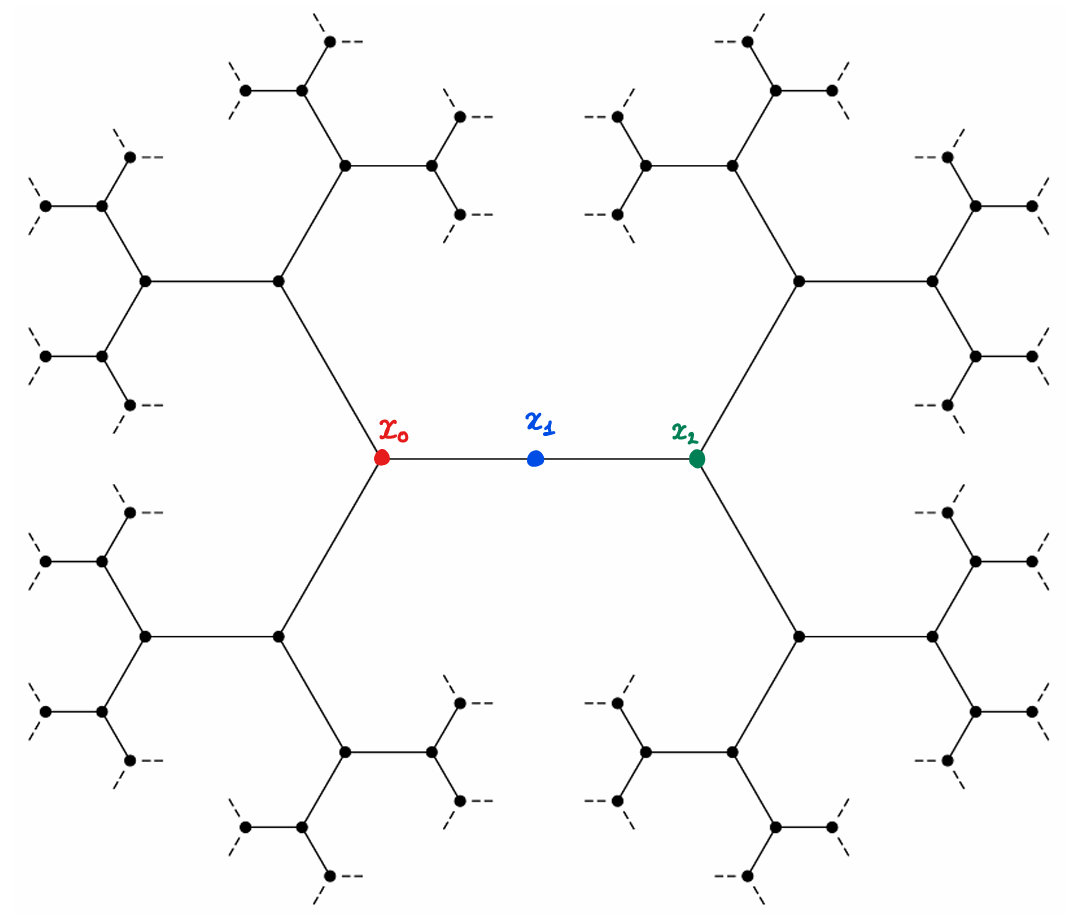
\includegraphics[scale=0.7]{BT-building for SL2.png}
                \captionof{figure}{Bruhat-Tits building of $\SL_2(\QQ_2)$}
            \end{tikzfigure}
            
            Parahoric subgroups of $\SL_2(\QQ_p)$ are conjugate to one of the following open compact subgroups:
            \begin{center}
                \begin{tabular}{cc}
                    $G_{x_0}=\begin{pmatrix} \ZZ_p & \ZZ_p \\ \ZZ_p & \ZZ_p \end{pmatrix}$ & $G_{x_0}^+=\begin{pmatrix} 1+p\ZZ_p & p\ZZ_p \\ p\ZZ_p & 1+p\ZZ_p \end{pmatrix}$ \\
                    
                    $G_{x_1}=\begin{pmatrix} \ZZ_p^\times & \ZZ_p \\ p\ZZ_p & \ZZ_p^\times \end{pmatrix}$ & $G_{x_1}^+=\begin{pmatrix} 1+p\ZZ_p & \ZZ_p \\ p\ZZ_p & 1+p\ZZ_p \end{pmatrix}$ \\
                    
                    $G_{x_2}=\begin{pmatrix} \ZZ_p & p^{-1}\ZZ_p \\ p\ZZ_p & \ZZ_p \end{pmatrix}$ & $G_{x_2}^+=\begin{pmatrix} 1+p\ZZ_p & \ZZ_p \\ p^2\ZZ_p & 1+p\ZZ_p \end{pmatrix}$.\\
                \end{tabular}
            \end{center}
            The corresponding reductive quotients are $$\mathrm{G}_{x_0}(\Fq) \cong \SL_2(\Fq), \mathrm{G}_{x_1}(\Fq) \cong \Fq^\times,\text{ and }\mathrm{G}_{x_2}(\Fq) \cong \SL_2(\Fq).$$
        \end{example}
    }
    

    % --- COLUMN 3: Local Langlands ---
    \column{0.25}
    \block{The parahoric restriction map}{
        For any parahoric subgroup $G_x$ and irreducible admissible representation $(\pi,V)$, the space of $G_x^+$-invariants $V^{G_x^+}$ is naturally a representation of the reductive quotient $\mathrm{G}_x(\Fq)$. This construction can be extended to a functor
        \begin{align*}
            \mathrm{res}^{G_x}: R(G) &\longrightarrow R(\mathrm{G}_x(\Fq))\\
            V&\longmapsto V^{G_x^+},
        \end{align*}
        where $R(G)$ and $R(\mathrm{G}_x(\Fq))$ are the vector spaces of formal complex linear combinations of irreducible representations of $G$ and $\mathrm{G}_x(\Fq)$, respectively. This functor is
        called the \textbf{parahoric restriction map}. 
    }
    \block{Unipotent representations}{
        In their groundbreaking work, Deligne and Lusztig classified the irreducible representations of finite groups of Lie type $\mathrm{G}(\Fq)$. They defined a special class of representations of geometric origin called \textbf{unipotent representations}, which are those that appear in the cohomology of Deligne--Lusztig varieties. 

        \textbf{Intuition:} The set of unipotent representations of $\mathrm{G}(\Fq)$ is a ``geometric completion" of the set of principal series representations. 
        \vspace{0.5cm}

        At the level of $p$-adic groups, we say that an irreducible admissible representation $(\pi,V)$ of $G$ is \textbf{unipotent} if there exists a parahoric subgroup $G_x$ such that $\mathrm{res}^{G_x}(V)$ contains a unipotent representation of $\mathrm{G}_x(\Fq)$. Since principal series representations of $\mathrm{G}(\Fq)$ are unipotent, Iwahori-spherical representations of $G$ are unipotent.
        
        \vspace{0.5cm}

        Unipotent representations of $G$ have many remarkable properties. For instance, under the LLC, they correspond to pairs $(\varphi,\phi)$ where $\varphi$ is trivial on the inertia subgroup $I_F$ of $W_F$. Equivalently, there is a bijection between
        \begin{align*}
            \left\{
            \begin{array}{c}
                \text{Unipotent irreducible} \\
                \text{admissible complex} \\
                \text{reps of } G(F)
            \end{array}
            \right\} 
            &\leftrightarrow
            \left\{
            \begin{array}{c}
                \text{Pairs } (x,\phi), \text{ where}\\
                x\in G^\vee(\CC)\text{ and}\\
                \phi \in \mathrm{Irr}\left(Z_{G^\vee}(x)/Z_{G^\vee}(x)^0\right)
            \end{array}
            \right\}.
        \end{align*}

        Moreover, the parahoric restriction functor $\mathrm{res}^{G_x}$ can be restricted to the space $R_{\mathrm{un}}(G)$ of virtual unipotent representations of $G$, giving the functor
        $$\mathrm{res}_{\mathrm{un}}^{G_x}: R_{\mathrm{un}}(G) \longrightarrow R_{\mathrm{un}}(\mathrm{G}_x(\Fq))$$
        whose image is the space of virtual unipotent representations of $\mathrm{G}_x(\Fq)$.
         

    }

    % --- COLUMN 4: Main Results/Visuals ---
    \column{0.25}
    \block{The nonabelian Fourier transform}{
        Lusztig further realised that there was a basis of $R_{\mathrm{un}}(\mathrm{G}(\Fq))$ with geometric significance arising naturally from the theory of character sheaves on the group $\mathrm{G}(\overline{\Fq})$. He called these basis elements \textbf{almost characters}. The change of basis transformation between irreducible characters and almost characters of $\mathrm{G}(\Fq)$ is called the \textbf{nonabelian Fourier transform} denoted by 
        $$\mathrm{FT}^{\mathrm{G}}: R_{\mathrm{un}}(\mathrm{G}(\Fq)) \longrightarrow R_{\mathrm{un}}(\mathrm{G}(\Fq)).$$
        %Moreover, Lusztig showed that this map is an involution and is Hermitian.
        \vspace{0.5cm}
        \begin{example}
            The group $\mathrm{G}(\Fq)=G_2(\Fq)$ has $10$ unipotent representations, often labelled as $\phi_{1,0}$, $\phi_{1,6}$, $\phi_{2,1}$, $\phi_{1,3}'$, $G_2[1]$, $\phi_{2,2}$, $G_2[-1]$, $\phi_{1,3}''$, $G_2[\theta]$ and $G_2[\theta^2]$. The nonabelian Fourier transform fixes $\phi_{1,0}$ and $\phi_{1,6}$, while it acts on the remaining $8$ representations as follows:
            \begin{tikzfigure}
                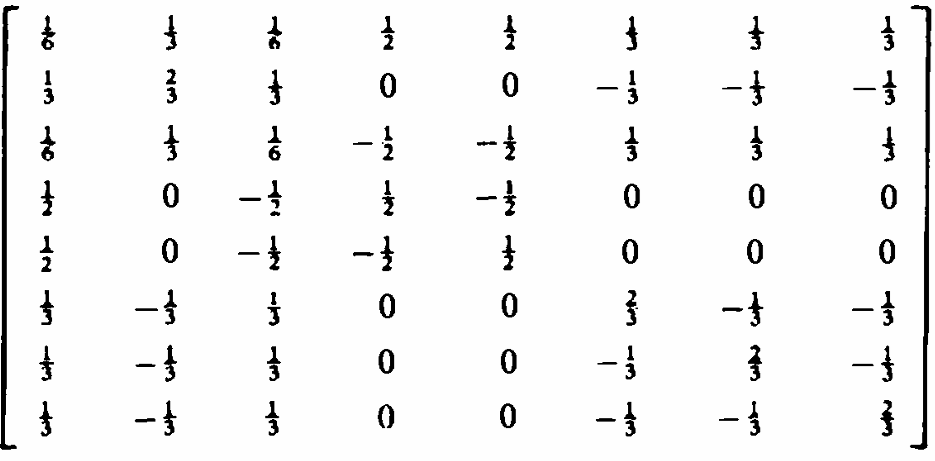
\includegraphics[scale=0.7]{fourier transform matrix.png}
                \captionof{figure}{Nonabelian Fourier transform matrix for $G_2(\Fq)$}
            \end{tikzfigure}
        \end{example}
    }
    \block{Main results}{
        It is conjectured that there is a \textbf{dual nonabelian Fourier transform} $\mathrm{FT}^{\vee}$ on $R_{\mathrm{un}}(G)$ for unipotent representations of $G$ compatible with the nonabelian Fourier transform $\mathrm{FT}^{\mathrm{G}_x}$ and unipotent parahoric restriction $\mathrm{res}_{\mathrm{un}}^{G_x}$ for all $x\in\mathcal{B}(G)$. Such a map has only been constructed for a certain subspace $R_{\mathrm{un},\mathrm{ell}}(G)$ of $R_{\mathrm{un}}(G)$, called the space of \textbf{elliptic unipotent representations}. 
        \vspace{0.5cm}
        \begin{conjecture}
            Up to certain roots of unity, the following diagram commutes for all $x\in\mathcal{B}(G)$:
            \[
                \begin{tikzcd}[ampersand replacement=\&]
                R_{\un,\text{ell}}(G) \arrow[r, "\FT^\vee_{\text{ell}}"] \arrow[d, "\res_{\un}^{G_x}"] \& R_{\un,\text{ell}}(G) \arrow[d, "\res_{\un}^{G_x}"] \\
                R_{\un}(\mathrm{G}_x(\Fq)) \arrow[r, "\FT^{G_x}"] \& R_{\un}(\mathrm{G}_x(\Fq)).
                \end{tikzcd}
            \]
        \end{conjecture}
        \vspace{0.5cm}
        \textbf{Known cases:} The conjecture above holds for $G$ of type $A_n$ (Aubert--Ciubotaru--Romano), $B_n$ (Moeglin--Waldspurger), $G_2$ (Ciubotaru--Opdam) and $F_4$ (L.B.). The other types remain an open problem.
    }

    
\end{columns}

\end{document}